In this chapter I'm going to contextualize the state of the art of my research work. 
Besides, I'll give explanation about the target to reach and the solution applied.\par
In our times a lots of businesses use Big Data for analysing and providing actionable knowledge.
Big Data is defined as large data sets collected from difference sources such as applications, social networks and websites.
For this, we are seeing nowadays a rapid growth of them which  causes a rise of redundancy and corrupted data.
The next consequence will be an accuracy reduction if models are built from them.
Data must be pre-processed before training, in order to reduce overfitting and improve accuracy of the final model.\newline
Another aspect to take in consideration is that a ML model trained with so many features it would be a black box, in which a lack of interpretability couldn't be able to explain the decisions taken by the AI.
So it's needed to care about interpretability in order to discard eventually confounding variables  which can suggest there is a correlation when in fact there is not, even if the model's accuracy is extremely high. \newline
\begin{figure}[H]
    \centering
    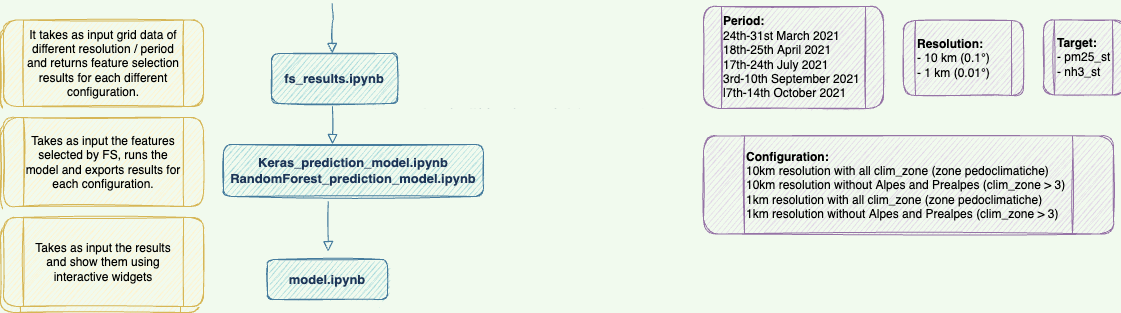
\includegraphics[scale=0.35]{images/overview _notebooks.png}
    \caption{}
    \label{fig:overview}
\end{figure}

For instance, a new paper by Alex DeGrave et al.\cite{degrave2021ai} shows that Deep Learning model trained with improper data was taking shortcuts in COVID-19 detection on radiographs because of position of certain markers rather than on the actual radiograph.
Therefore, the key to increase interpretability of a given model is to wonder if given factor should drive the final decision.\par
In this context, in which the black-box nature of ML algorithms raises ethical and judicial concerns inducing lack of trust\cite{9141213}, Explainable Artificial Intelligence aims to create a model fully interpretable.
Before the advent of XAI, scientific community was focused on the predictive power of algorithms rather than the understanding behind these predictions.
This need for trustworthy for high performing models led to  Interpretable Artificial Intelligence (XAI), a field focused on the interpretation of how AI systems take decision.
This issue about interpretability and clearness are being identified increasingly as critically significant nowadays. 
This is consistent with what could be found by searching in Google Trends, where the trend of 'Explainable Artificial Intelligence' grew up in the last 3 years, while the curve of  'AI' seems to have reached a saturation state (Figure \ref{fig:AI_XAI}).
Interpretable Artificial Intelligence (or Interpretable Machine Learning) helps to understand how ML algorithms make prediction, with the usage of Feature Selection methods for clarify model’s decision.
Feature selection can give relevant explanations by quantifying the influence of each independent variable with a score.
In order to do that, before developing a predictive model, feature selection is a needed step for reducing the number of input variable. \newline
Nowadays, with the large amount of volume and variety in Big Data, FS is becoming increasingly an essential pre-processing step in machine learning algorithms \cite{kamolov2021feature}.
It is desirable to both reduce the computational cost of modelling and, in some cases, to improve the performance of the model.\newline
\begin{figure}[H]
    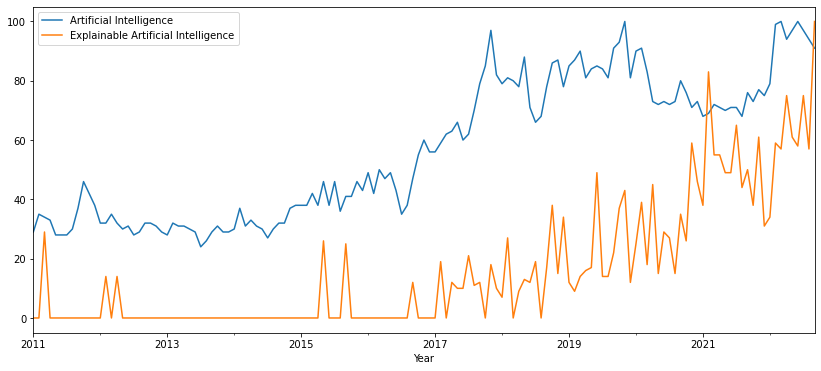
\includegraphics[scale=0.50]{images/AI_XAI.png}
    \caption{This plot is provided by Google Trends in which are shown the scores obtained by 'Artificial Intelligence' and 'Interpretable Artificial Intelligence' trends in the period between 2011 and 2022.}
    \label{fig:AI_XAI}
\end{figure}
\bigbreak
Inside the D-DUST project this step aims to provided a weighted score of each environmental variable with respect to the pollutants emitted by intense agricultural through regression predictive modeling.\newline
\par
Due to the fact there isn’t a best feature selection technique, I performed and combined different supervised methods. 
\bigbreak
According to the above, my work comes on this scenario, having the aim to pre-process geospatial data in order to highlight the most weighted input variable that affect the pollutants related to intense agriculture and farming.\newline
The final goal of my research is to implement a Machine Learning model capable of predicting pollutant locally with better precision than global scale. 




